\documentclass[cfr,biber]{now-journal}
\usepackage{epstopdf}

\title{Critical Finance Review Figure and Table Examples}

\author{Alet Heezemans}

\affil{Now Publishers}

\articledatabox{ISSN 2164-5744 ; DOI 10.1561/104.XXXXXXXX\\
\copyright \ A. Heezemans}

\keywords{CFR articles must always contain keywords}
\keywords[JEL]{CFR articles must always contain JEL codes}

\begin{document}

\begin{abstract}
Below are given: one example of a figure with a caption, a source, a description and an interpretation; one example of a table that breaks over two pages with a caption, a note, and a description; and one example of a table on a single page with a caption, a note, and an interpretation. Please consult these examples when typesetting figures and tables for the \itshape{Critical Finance Review}.
\end{abstract}


\begin{figure}[p]  %F1
 \centerline{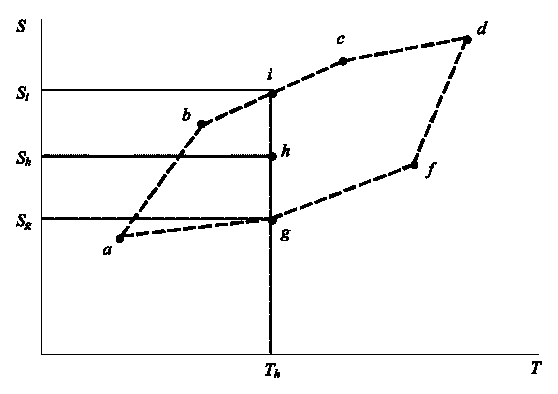
\includegraphics{f01}}
\Source{Adapted from a source.}
\caption{Contract zone.\label{fig1}}
\Description{The sample includes all common stocks on CRSP with current-month returns
(Return, {\%}) and beginning-of-month market value, book-to-market
equity, and lagged 12-month returns.}
\Interpretation{This table summarizes Fama-MacBeth cross-sectional regressions
(average slopes, R$^{2}$s, and number of stocks) when monthly
returns (in {\%}) are regressed on lagged firm characteristics.
}
\end{figure}


\begin{table}[p]%T1
\begin{center}
 \caption{Descriptive statistics, 1964--2013.}
 {\fontsize{10}{12}\selectfont\begin{tabular}{@{}ld{6,4}d{5,4}d{5,4}@{}}
 \toprule
& \multicolumn{1}{c}{All schools} & \multicolumn{1}{c}{Public} & \multicolumn{1}{c}{Community} \\
Variable & \multicolumn{1}{c}{($N= 132$)}& \multicolumn{1}{c}{($N=80$)} & \multicolumn{1}{c}{($N=52$)} \\
 \midrule
Average salary*& 47317.52& 56481.86& 33218.52 \\
& (13810.29)& (9282.984)& (4689.734) \\[2pt]
Average teaching experience*& 11.386 & 16.125 & 4.096 \\
& (6.682) & (2.999) & (3.368) \\[2pt]
{\%} Teachers with masters*& 36.451 & 47.144 & 20 .000 \\
& (21.208) & (17.691) & (14.672) \\[6pt]
RCP**& 0.531& 0.649& 0.351 \\
& (0.32)& (0.33)& (0.20) \\[2pt]
Private enroll/public enroll*& 16.433& 15.220& 18.298 \\
& (9.09)& (10.14)& (6.85) \\[2pt]
Community school& 0.394& \multicolumn{1}{c}{---} & \multicolumn{1}{c}{---} \\
& (0.49)& &  \\[2pt]
Enrollment**& 387.212& 439.663& 306.519 \\
& (200.45)& (192.65)& (186.46) \\[2pt]
Administrative expenses ({\%})**& 11.230& 5.573& 19.933 \\
& (16.29)& (1.21)& (23.50) \\[2pt]
Test performance*& 0.000& 0.137& -0.210 \\
& (1.00)& (1.09)& (0.80) \\[2pt]
Population/Sq. Mile**& 1690.467& 1607.043& 1818.811 \\
& (1129.26)& (1289.58)& (819.63) \\[2pt]
Median income ({\$}000s)**& 38.909& 38.174& 40.039 \\
& (3.96)& (4.65)& (2.14) \\[2pt]
{\%} College**& 22.080& 20.350& 24.740 \\
& (6.80)& (7.37)& (4.76) \\[2pt]
Median house price ({\$}000s)& 102.825& 101.188& 105.344 \\
& (17.61)& (20.46)& (11.71) \\[2pt]
Median rent**& 502.644& 487.963& 525.231 \\
& (63.77)& (70.83)& (42.64) \\[2pt]
Median wage**& 750.076& 733.375& 775.769 \\
& (113.47)& (128.45)& (80.01) \\[2pt]
{\%} Minority**& 22.906& 20.835& 26.092 \\
& (12.15)& (14.34)& (6.61) \\[2pt]
Median age**& 36.630& 37.046& 35.990 \\
& (2.15)& (14.34)& (6.61) \\
 \bottomrule
\multicolumn{4}{r@{}}{({\it Continued})}
\end{tabular}}
 \end{center}
\end{table}

\setcounter{table}{0}

\begin{table}[t]%T1
 \caption{({\it Continued})}
{\fontsize{10}{12}\selectfont\begin{tabular}{@{}ld{6,4}d{5,4}d{5,4}@{}}
 \toprule
& \multicolumn{1}{c}{All schools} & \multicolumn{1}{c}{Public} & \multicolumn{1}{c}{Community} \\
Variable & \multicolumn{1}{c}{($N= 132$)}& \multicolumn{1}{c}{($N=80$)} & \multicolumn{1}{c}{($N=52$)} \\
 \midrule
{\%} Single mom**& 12.126& 11.366& 13.294 \\
\phantom{Administrative expenses ({\%})**} & (3.09)& (3.61)& (1.47) \\[2pt]
{\%} Below poverty& 9.405& 9.573& 9.146 \\
& (1.85)& (2.16)& (1.22) \\[2pt]
Crime Rate**& 3.832& 3.157& 4.870 \\
& (1.72)& (1.69)& (1.16) \\
 \bottomrule
\end{tabular}}
\Note{The above figures are means for the sample or subsample noted with standard
deviations in parentheses. Significant differences in means across school type are
denoted **for significance at the 5{\%} level and *for significance at the 10{\%}
level.}
 \Description{The sample includes all common stocks on CRSP with current-month returns
(Return, {\%}) and beginning-of-month market value, book-to-market
equity, and lagged 12-month returns.\label{tab1}}
\end{table}


\begin{table}[p]%T2
\begin{center}
 \caption{Fractional logit results.\label{tab2}}
 {\fontsize{9}{11}\selectfont\tabcolsep15pt\begin{tabular}{@{}ld{2,5}d{2,3}@{}}
 \toprule
& \multicolumn{1}{c}{Coefficient} & \multicolumn{1}{c@{}}{Marginal} \\
Variable & \multicolumn{1}{c}{(std. error)} & \multicolumn{1}{c@{}}{effect} \\
 \midrule
Intercept& 23.195 & \multicolumn{1}{c}{---} \\
& (39.229)&  \\[2pt]
Private enroll/public enroll& 0.098* & 0.024 \\
& (0.052) &\\[2pt]
Community school& -2.173^{**} & -0.495 \\
& (0.218) &\\[2pt]
Enrollment (log)& -0.051 & -0.012 \\
& (0.172) &\\[2pt]
Administrative expenses ({\%})& -0.008 & -0.002 \\
& (0.007) & \\[2pt]
Test performance& -0.279^{**} & -0.068 \\
& (0.118) & \\[2pt]
Population/sq. mile (log)& 0.670 & 0.164 \\
& (0.495) & \\[2pt]
Median income (log)& -6.545 & -1.603 \\
& (4.914) &\\[2pt]
{\%} College& -0.067^* & -0.017 \\
& (0.037) & \\[2pt]
Median house price (log)& -1.668 & -0.409 \\
& (1.892) & \\[2pt]
Median rent (log)& 10.939^{**} & 2.679 \\
& (4.664) & \\[2pt]
Median wage (log)& -0.605 & -0.148 \\
& (0.935) & \\[2pt]
{\%} Minority& -0.015 & -0.004 \\
& (0.039) & \\[2pt]
Median age& 0.065 & 0.016 \\
& (0.056) & \\[2pt]
{\%} Single mom& -0.251 & -0.062 \\
& (0.167) & \\[2pt]
{\%} Below poverty& -0.143 & -0.035 \\
& (0.135) & \\[2pt]
Crime rate ({\%})& 0.107 &  \\
& (0.137) & 0.026 \\
 \bottomrule\\[-6pt]

\end{tabular}}
\end{center}
\Note{$N=132$. The dependent variable is RCP;
$^{**}$indicates significance at the 5 {\%} level and $^*$indicates significance at the
10{\%} level.}
\Interpretation{These values are useful for interpretation and appropriate for
comparison to OLS results. Although we estimated an OLS regression using the same
variables, we prefer results from the flogit specification of the model.}
\end{table}
\end{document}